\documentclass[a4paper,10pt]{article}
\usepackage[utf8]{inputenc}
\usepackage[english]{babel}
\usepackage{float}
\usepackage{graphicx}
\usepackage{caption}
\usepackage{subcaption}
\usepackage{amsmath}
\usepackage{multirow}

%opening
\title{Deep convolutional networks for protein fold quality assessment}
\author{}

\begin{document}

\maketitle

\begin{abstract}

\end{abstract}

\section{Introduction}
Proteins are the cogs of the cell machinery. In order to understand responses of a cell to the external stimuli given their internal state, we
have to be able to predict the function of the proteins expressed in a cell. The current paradigm dictates that the function 
of a protein is determined mainly by its structure that dictates its interactions with other molecules present in a cell. 
Therefore the problem of a protein structure prediction (protein folding) is one of the limiting factors in understanding and designing living
organisms.

The progress in the field of protein folding is monitored by Critical Assessment of protein Structure Prediction (CASP) \cite{moult1995large}. This 
is a community-wide experiment to evaluate the protein folding prediction methods. Every method participating in this competition has a pipline
that includes sampling and quality assessment (QA) steps. During the sampling part, the candidate conformations of a protein are generated. The 
QA part of an algorithm tries to select the candidates closest to the unknown native structure.

In this paper we explore the application of deep learning, a new machine learning technique to the protein decoys quality assessment problem. 
Deep learning (DL) is a popular  approach in the field of machine learning, which recently gained considerable interest 
in the research community \cite{lecun2015deep}, particularly in computer vision and image recognition. 
Unlike previous ‘shallow’ approaches, DL tries to learn hierarchical representation of the 
data in hand. It alleviates the need for feature extraction that constituted the bulk of the work done by researchers. 

Recently, DL was applied to biological data and yielded remarkable results in the human splicing code prediction \cite{xiong2015human}, 
identification of DNA- and RNA-binding  motifs \cite{alipanahi2015predicting} and predicting the effects of non-coding 
DNA variants at single nucleotide polymorphism 
precision \cite{zhou2015predicting}. These successes have one thing in common: they do not introduce any features 
between the raw data and the deep learning model. 

\subsection{Related work}
Deep learning methods were also applied in the field of structure quality assessment \cite{}. In particular, 
DeepQA \cite{} used 9 scores from other QA estimators and 
7 physico-chemical feature estracted from a structure as the input features to the deep boltzman machine \cite{}. 
In the DL-PRO algorithm \cite{}, authors first compute contact maps of the decoys and compress them using PCA. 
The vectors from PCA are then fed into an autoencoder to predict the score of the decoy. 
The authors that apply the deep learning methods use them as the ordinary 'shallow' classifiers. 
Therefore they do not get all the advantages these new techniques offer.


\section{Materials and Methods}




\subsection{Datasets}
To train and assess our method we used the datasets of protein decoys from the CASP competition. 
We took the datasets CASP7 - CASP10 as the training set and the CASP11 dataset as the test set.
We optimized side chain conformation of the training and test sets using SCWRL program \cite{}.
The training and test sets have 564 and 83 targets correspondingly. For each target these datasets have 
on average x decoys. The native structures were not included in the datasets nor during the training procedure
neither during the testing phase. The distribution os target sequence lengths are shown on Fig. \ref{Fig:dataLengthDist}. We see,
that these two datasets cover the same interval of sequence lengths. However, to ensure that the training 
and test sets are significantly diverse we aligned all the sequences from the test set agains all the training 
set sequences using blasp tool \cite{}. The most significant alignments are shown in the Table \ref{Tbl:datasetsSimilarity}.
We see that less than 15\% of the targets in the test set have similar sequence stretches to the targets in the training set.

To assess the structural similarity of the two datasets we found the pfam family of each target in the training and the 
test sets and computed the overlap between the families in both datasets. We used HMMER tool with the e-value cutoff 1.0 to 
find the pfam family of a target \cite{}.

\begin{figure}[H]
    \centering
    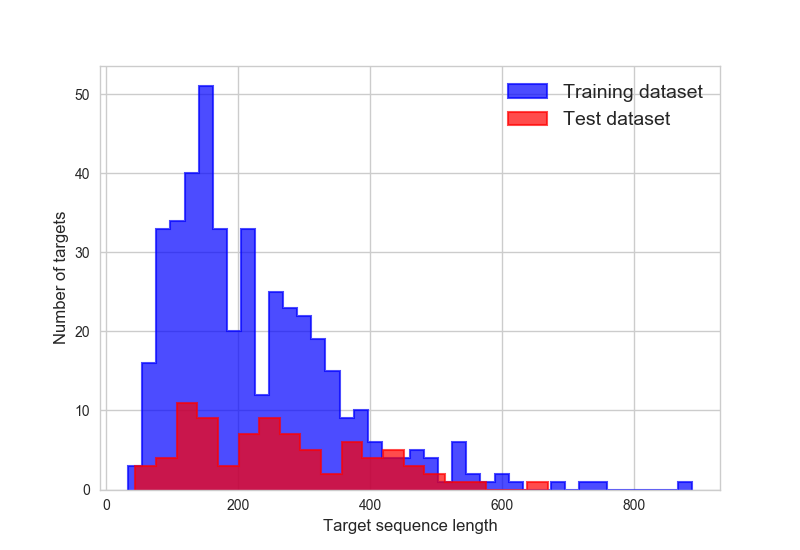
\includegraphics[width=\linewidth]{Fig/datasetLengthDistributions.png}
    \caption{The distributions of sequence lengths for targets in training set(blue) and test set(red).}
    \label{Fig:dataLengthDist}
\end{figure}

\begin{table}[H]
\begin{center}
\begin{tabular}{ c | c | l }
    
    Test set id & Closest training set id & E-value \\
    \hline
    T0768 & T0690 & 2.7e-13\\
    T0770 & T0645 & 1.79e-13\\
    T0772 & T0518 & 1.89-07\\
    T0776 & T0707 & 3.98e-05\\
    T0783 & T0699 & 1.19e-22\\
    T0798 & T0308 & 9.57e-06\\
    T0813 & T0398 & 2.45e-05\\
    T0819 & T0636 & 8.66e-15\\
    T0854 & T0324 & 2.13e-13\\
    %T0792 & T0375 & 0.013\\
    %T0786 & T0204 & 0.082\\
    %T0848 & T0542 & 0.087\\
    %T0777 & T0685 & 0.039\\
    %T0816 & T0473 & 0.0077\\
    %T0814 & T0758 & 0.033\\
    
\end{tabular}
    
    \caption {The closest homologs from training and test sets. The search was performed using blastp tool. The database was constructed from 
    the training set sequences; test sequences were queried against this database. We used 1e-4 e-value cutoff to filter only significant 
    alignments.}
    \label{Tbl:datasetsSimilarity}
\end{center}
\end{table}

\subsection{Input and Model}
\begin{figure}[H]
    \centering
    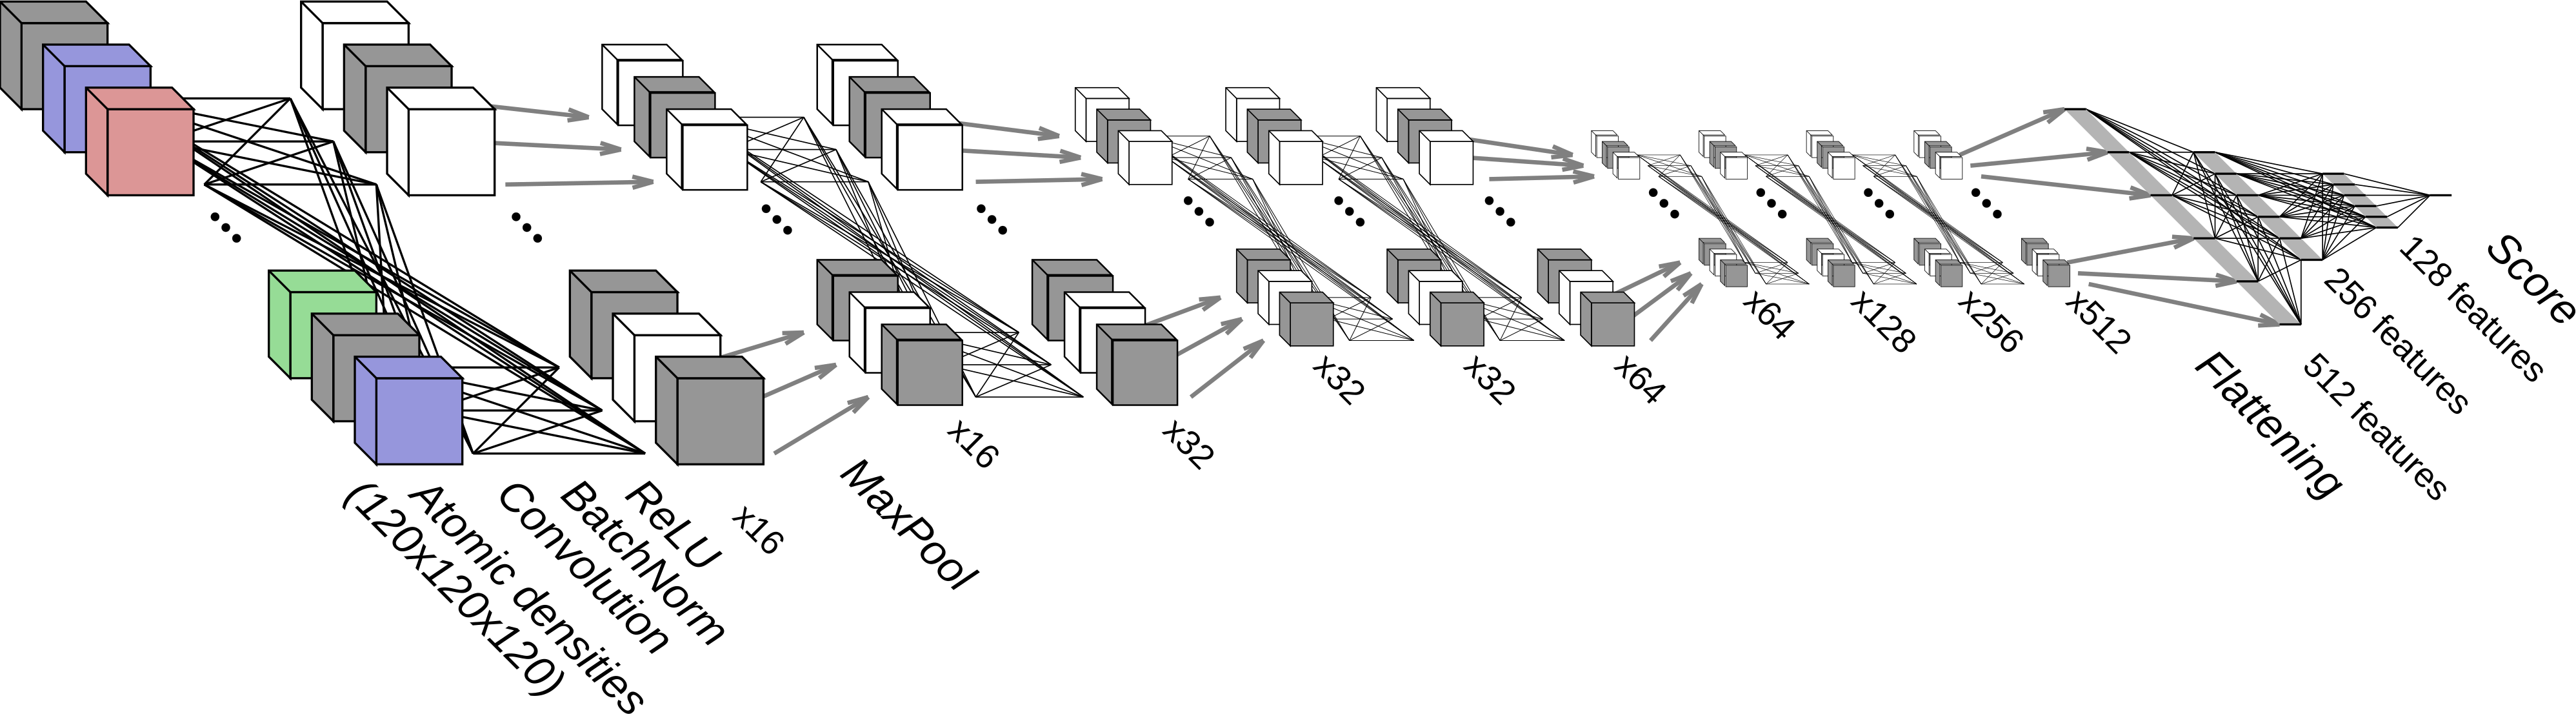
\includegraphics[width=\linewidth]{Fig/ConvnetDiagramV1.png}
    \caption{The schematic representation of the convolutional neural network architecture used in this work.}
    \label{Fig:CNNModel}
\end{figure}
The schematic representation of the model architecture is shown on the Fig \ref{Fig:CNNModel}. 
It is comprised of three blocks of alternating convolutional, 
volumetric batch normalization and ReLU layers and three 
fully connected layers with ReLU nonlinearities. The final output of the network is a single number, 
that is interpreted as a score of an input structure.
The input of the model is the density maps of atom types in a structure. We used 11 types of atoms shown in the Table \ref{Tbl:atomTypes}. 
Each atom type was projected on the corresponding grid and served as an input of the model. 
The density of an atom was modeled using the function: 
$$
\rho(r) =  \begin{cases}
               e^{-\frac{r^2}{2}}&r\leq 2.0\AA~\\
               0                 &r>2.0\AA~\\
            \end{cases}
$$
\begin{table}[H]
\begin{center}
\begin{tabular}{ c | l | l }
    
    Type & Description & Atoms \\
    \hline
    1 & Sulfur containing atoms & CYSSG, METSD, MSESE \\ \hline
    2 & Amide nitrogens & ASNND2, GLNNE2, backbone N \\ \hline
    3 & Aromatic nitrogens & HISND1, HISNE2, TRPNE1 \\ \hline
    4 & Guanidine nitrogens & ARGNH1, ARGNH2, ARGNE \\ \hline
    5 & Nitrogen with three hydrogens & LYSNZ \\ \hline
    6 & Carboxyl oxygen & ACEO, ASNOD1, GLNOE1, backbone O \\ \hline
    7 & Oxygen in hydroxyl group & SEROG, THROG1, TYROH \\ \hline
    8 & Oxygen in carboxyl group and terminus oxygen & ASPOD1, ASPOD2, GLUOE1, GLUOE2, \\
     & &  O-terminal, OT2-terminal, OXT-terminal \\ \hline
    9 & Sp2 carbon & ARGCZ, ASPCG, GLUCD, ACEC, \\
     & & ASNCG, GLNCD, backbone C \\ \hline
    10 & Aromatic carbon & HISCD2, HISCE1, HISCG, PHECD1 \\
     & & PHECD2, PHECE1, PHECE2, PHECG \\ 
     & & PHECZ, TRPCD1, TRPCD2, TRPCE2 \\
     & & TRPCE3, TRPCG, TRPCH2, TRPCZ2 \\
     & & TRPCZ3, TYRCD1, TYRCD2, TYRCE1 \\
     & & TYRCE2, TYRCG, TYRCZ \\ \hline
    11 & Sp3 carbon & ALACB, ARGCB, ARGCG, ARGCD \\
     & & ASNCB, ASPCB, GLNCB, GLNCG \\
     & & GLUCB, GLUCG, HISCB, HISCB \\
     & & ILECB, ILECD1, ILECG1, ILECG2 \\
     & & LEUCB, LEUCD1, LEUCD2, LEUCG \\
     & & LYSCB, LYSCD, LYSCG, LYSCE \\
     & & METCB, METCE, METCG, MSECB \\
     & & MSECE, MSECG, PHECB, PROCB \\
     & & PROCG, PROCD, SERCB, THRCG2 \\
     & & TRPCB, TYRCB, VALCB, VALCG1 \\
     & & VALCG2, ACECH3, THRCB, CYSCB \\
     & & backbone CA \\ \hline
    
\end{tabular}
    
    \caption {Atom types used in this work. In the atom notation the first three letters are the name of an aminoacid and the rest is 
    the atom name in the PDB format \cite{}}.
    \label{Tbl:atomTypes}
\end{center}
\end{table}
Figure \ref{Fig:atomic_densities} shows an example of atomic densities. 
The protein used for visualization has PDB code 5eh6. Only non-zero densities are shown.

\begin{figure}[H]
    \centering
    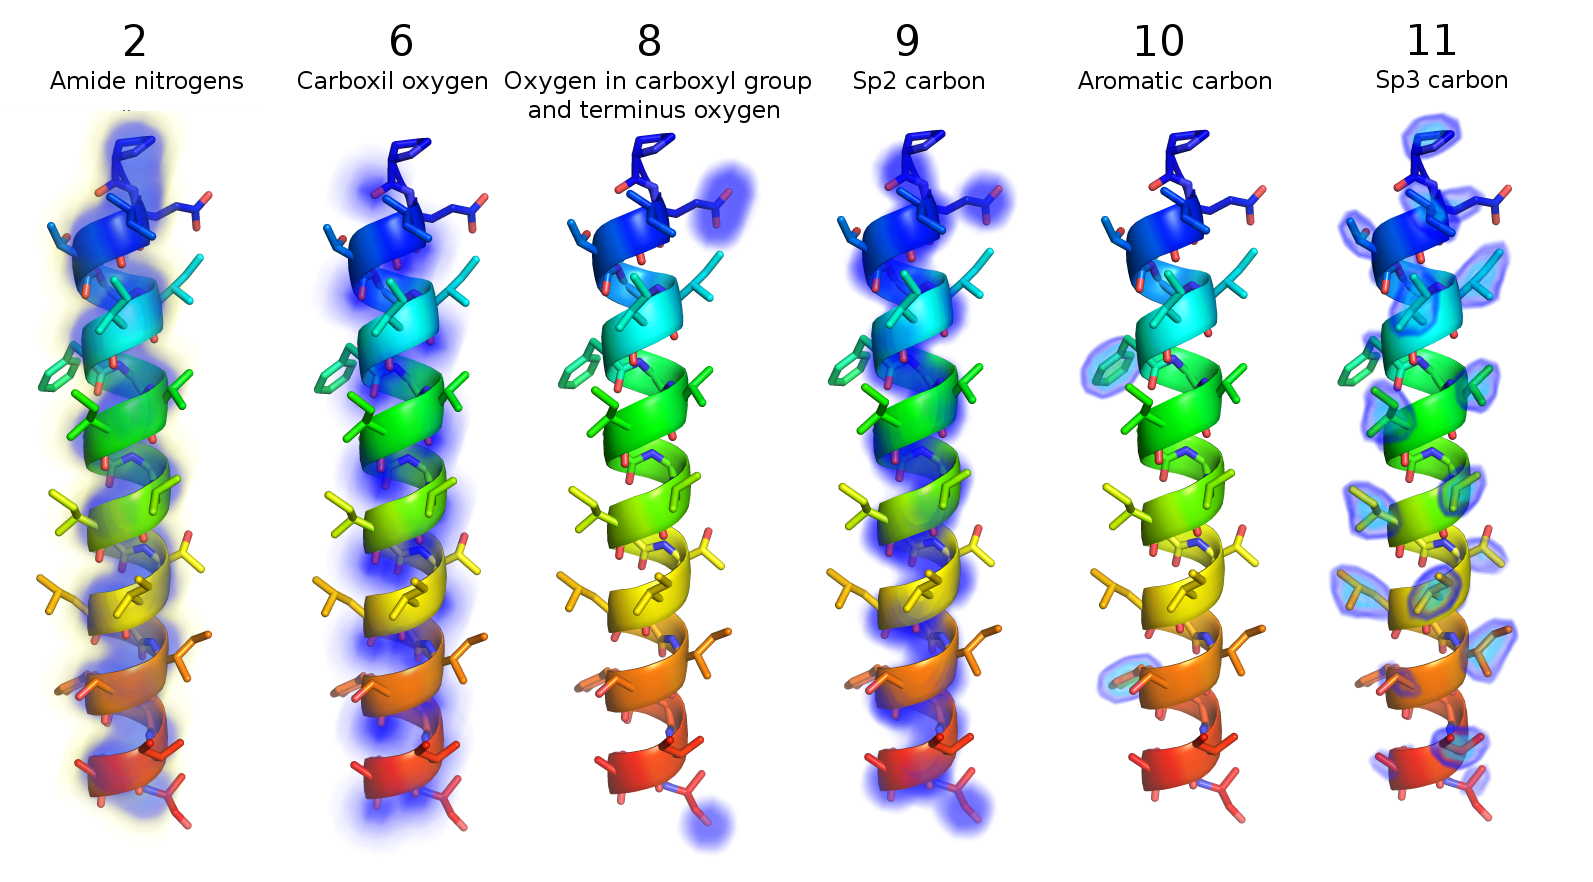
\includegraphics[width=\linewidth]{Fig/atomic_densities.png}
    \caption{The example of the representation of a protein using atomic densities. The density map is 
    shown using the volumetric rendering plugin for PyMol. The pdb-code of the protein used for this visualization is 5eh6.}
    \label{Fig:atomic_densities}
\end{figure}

\subsection{Loss functions}
We evaluated two scoring functions: linear regression and ranking scoring function. 
Let a decoy representation be denoted as $x_i$ and therefore the output
of the network on this decoy will be $f(x_i)$. Next, let $y_{ij}$ be the ordering coefficient of the two decoys we pick: 
$$
y_{ij} = \begin{cases}
               1& gdtts_i \leq gdtts_j \\
               -1& gdtts_i > gdtts_j \\
            \end{cases}
$$
Here $gdtts_i$ is the GDT-TS score of the $i$-th decoy. In principle, any target function can be chosen. 
The pairwise ranking scoring function has the following expression:

$$ L_{ij} = w_{ij} \cdot \max \left[ 0, 1 - y_{ij} \left( f \left( x_i \right) - f \left( x_j \right) \right) \right] $$

the term $w_{ij}$ represents an example weight:

$$
w_{ij} = \begin{cases}
               1& \left| gdtts_i - gdtts_j \right| > threshold \\
               0& otherwise \\ 
            \end{cases}
$$

where the $threshold$ is set to 0.1{\AA}. If the two decoys are too similar, 
we avoid scoring them against each other during the training, because it introduces 
the noise into the gradient and prevents optimization.


During the training procedure we load several decoys (batch) into memory and evaluate the model on them. 
Afterwards, we compute the average loss for the batch:
$$ L = \frac{1}{N} \sum_{i=1,j=1, i \neq j}^{M} L_ij $$ 
where $N$ is the number of pairs of decoys with the $w_{ij} > 0$ and $M$ is the number of decoys in a batch.

\subsection{Evaluation criteria}
We evaluated our algorithm using the correlation coefficients, Z-score and loss criterions. The correlation coefficents 
were computed between the score of 
our model and GDT-TS metric for all the decoys of each target protein in a test set and then averaged. 
The Z-score is the deviation of the score of 
the best decoy for a certain protein and average decoy score for this protein:
$$ 
Z-score = \frac{f( argmin(gdtts(x_i)) ) - <f(x)>}{std.dev.f(x)}
$$ 
the best decoy is the one with the lowest GDT-TS score. 
The loss criterion is the deviation of the GDT-TS of the best decoys for a protein from the GDT-TS score of the decoy with the lowest score:
$$ 
Loss = | max_i( gdtts_i ) - gdtts( argmin(f(x_i) ) |
$$ 

\subsection{Optimization and dataset sampling}
The optimization procedure of deep convolutional networks usually is stochastic: the function value and gradient 
is estimated on a small subset (batch) of all the training 
examples. We used the batch of size 10 due to the memory limitations. Afterward the parameters of the model are 
changed in the direction of the estimated gradient.
The parameter update step was performed using the Adam algorithm \cite{}. 

The dataset was sampled in the following way: first we chose a random protein from the dataset, then we sample decoys of this protein. 
The procedure is repeated for all the 
proteins in a dataset. One pass through all the proteins in a dataset is called epoch. 
The decoys are sampled in a homogeneous way: we divide all the decoys into $M$ clusters by the value of GDT-TS score. 
Precisely, the decoy $i$ belongs to the cluster  
number $ \left[ \frac{\max(gdtts) - gdtts_i}{\max(gdtts) - \min(gdtts)} \right] + 1$, where $\max(gdtts)$ and $\min(gdtts)$ 
are computed for all the decoys of 
the chosen protein. If there are empty clusters, then we take secon decoys from each non-empty and so on until we filled the batch. 
At the end of each epoch we randomly
shuffle the order of protein and the order of decoys in each cluster. 

Each decoy from the selected batch is randomly rotated and translated. The rotations are sampled uniformly \cite{}. The translation are chosen
in such a way, that the bounding box of the translated protein lies within the box of the size 120x120x120\AA. 

To select the final model we randomly divided the training set into training and validation subsets. The validation subset consists of 
35 targets and their decoys. This subset was not sampled during the training. 
Figure \ref{Fig:TrainingLoss} shows the Kendal tau, Pearsor R coefficients and the loss on the vaidation subset. 
The final model was chosen according to the minimum loss (epoch 40).
\begin{figure}[H]
    \centering
    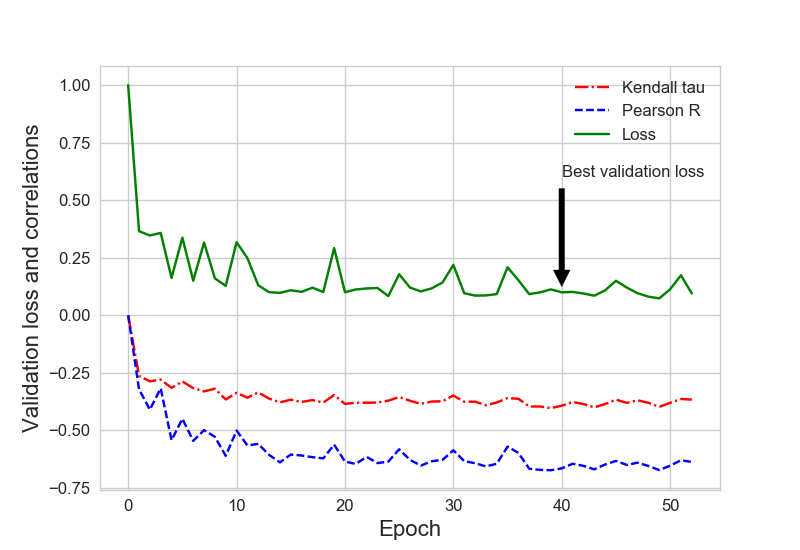
\includegraphics[width=\linewidth]{Fig/kendall_validation.png}
    \caption{The loss, Kendal tau and Pearson R coefficients evaluated on the validation subset during the training procedure. The epoch 
    denotes that all the targets in the training subset were sampled.}
    \label{Fig:TrainingLoss}
\end{figure}

The table \ref{Tbl:TrainingResults} summarizes the performance metrics on the training and validation sets for the model at epoch 40.

\begin{table}[H]
\begin{center}
\begin{tabular}{ c | c | c | c | c }
    Data subset & Loss & Pearson & Spearmann & Kendall \\
    \hline
    Training set     &0.146 &0.71 &0.61 &0.45 \\
    Validation set   &0.135 &0.71 &0.59 &0.44 \\ \hline

\end{tabular}
  \caption {Results of the model from epoch 40 on the training and validation subsets.}
    \label{Tbl:TrainingResults}
\end{center}
\end{table}

\section{Results}
During the training of the model we randomly sampled rotational and translational degrees of freedom of a decoy structure. Ideally, we 
want the score assigned by the model to a decoy to be invariant under these transformations. However Fig \ref{Fig:ScoreDistribution} 
shows that the distribution
of scores under rotations and translations follows the gaussian distribution. Therefore, to approximate the average score of a decoy we 
sample a score under random translation and rotation 20 times for each decoy in the test set. The final score is then the average of these 
samples.

\begin{figure}[H]
    \centering
    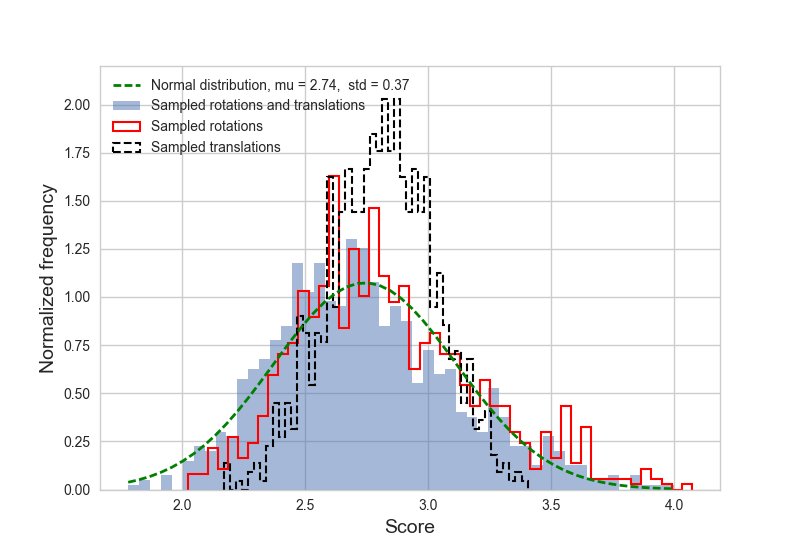
\includegraphics[width=\linewidth]{Fig/sampling_dist.png}
    \caption{The distribution of scores under random translations and rotations of the decoy LOOPP\_TS1 for the target T0342. The distributions 
    os scores under rotations only and translations only are shown with the dashed and solid lines respectively.
    The normal distribution fitted into the sampled scores under both rotations and translations is show with the dashed line. 
    The parameters of the normal distribution are: the average $\mu = 1.38$ and the standard deviation $\sigma = 0.42$.}
    \label{Fig:ScoreDistribution}
\end{figure}


Table \ref{Tbl:TestResults} shows the comparisson of our model with the state of art methods used for the decoy quality assessement. 
To evaluate the performance we used CASP11 stages 1 and 2 datasets. 
These datasets were preprocessed using SCWRL program to optimize side-chains. 

\begin{table}[H]
\begin{center}
\begin{tabular}{ c | c | c | c | c }
    \multicolumn{5}{ c }{Stage 1} \\ \hline

    QA method & Loss & Pearson & Spearmann & Kendall \\
    \hline
    ProQ2   &0.090 &0.643 &0.506 &0.379 \\
    Qprob   &0.097 &0.631 &0.517 &0.389 \\
    \textbf{3DCNN}   &\textbf{0.072} &0.530 &0.415 &0.318 \\
    RWplus  &0.135 &0.536 &0.433 &0.433 \\ \hline
    
    \multicolumn{5}{ c }{Stage 2} \\ \hline
    
    ProQ2   &\textbf{0.058} &0.372 &0.366 &0.256 \\ 
    Qprob   &0.068 &0.381 &0.387 &0.272 \\
    \textbf{3DCNN}     &\textbf{0.064} &\textbf{0.415} &\textbf{0.402} &\textbf{0.283} \\
    RWplus  &0.084 &0.295 &0.314 &0.220 \\ \hline

\end{tabular}
    
    \caption {Results of our method(3DCNN) and the other state-of-art quality assessment programs on the CASP11 dataset Stage 1 and 2.
            Table shows the absolute average values of correlation coefficients. The averaging was performed for each target in the 
            dataset. Afterwards all the values were averaged over all the targets.}
    \label{Tbl:TestResults}
\end{center}
\end{table}

\section{Analysis}


\section{Discussion}

\bibliography{citations.bib}{}
\bibliographystyle{plain}


\end{document}
